\documentclass{article}
\usepackage[utf8]{inputenc}
\usepackage{amsfonts} 
\usepackage{minted}
\usepackage{graphicx}
\graphicspath{ {./} }

\title{DE Assignment}
\author{Kirill Ivanov}
\date{October 2020}

\begin{document}

\maketitle

\section{Part I}
\subsection{Exact solution (4th variant)}
$$ 2x^3+2\frac{y}{x}=y' $$ We can rewrite it as:
$$ y'-2\frac{y}{x}=2x^3 $$ It is a linear F.O. O.D.E with non-homogeneous coefficients. Let’s solve a complementary equation:
$$ y'-2\frac{y}{x}=0 $$ After some mathematical operations we get:
$$ \frac{y'}{y}=\frac{2}{x} $$ (we assume that $ y \neq 0 $  Also, $ y = 0 $ is not a trivial solution). Using the property of differential we find: $$ \frac{dy}{y}=2\frac{dx}{x} $$
Integrating it we get \\ 
\begin{center}
    $ y = C_1 x^2, C_1 \in \mathbb{R} $ and $ C_1 \neq 0 $
\end{center} 

\begin{center}
    $ C_1 \rightarrow C_1(x) $, so $$ y' = C'_1(x)x^2 + 2C_1(x)x $$   
\end{center} 

Substituting obtained values of $ y $ and $ y' $ into the rewritten original equation we get
$$ C'_1(x)x^2 + 2C_1(x)x-2\frac{C_1 x^2}{x}=2x^3 $$ From this we get $$ C'_1(x) = 2x $$
Integrating this we obtain 
\begin{center}
$ C_1(x)=x^2+C, x^2 \neq C $ (as $ C_1 \neq 0 $) 
\end{center}
Now we can find y: 
\begin{center}$ y = x^4 + x^2C, x^2 \neq C $ and $ x \neq 0 $ (since $ y \neq 0 $)
\end{center}
This is the exact solution. \\
Now we need to express $ C $ in terms of $ x_0, y_0 $.
We have $$ y_0 = y(x_0) = x_0^4 + x_0^2 C $$ so  $$ C = \frac{y_0}{x_0^2}-x_0^2 $$
Substituting it into the exact solution we find: $$ y = x^2(x^2+\frac{y_0}{x_0^2}-x_0^2) $$ This formula is ready for our application.

\section {Part II}
\subsection{Plots created by the program (approximations and LTEs)}
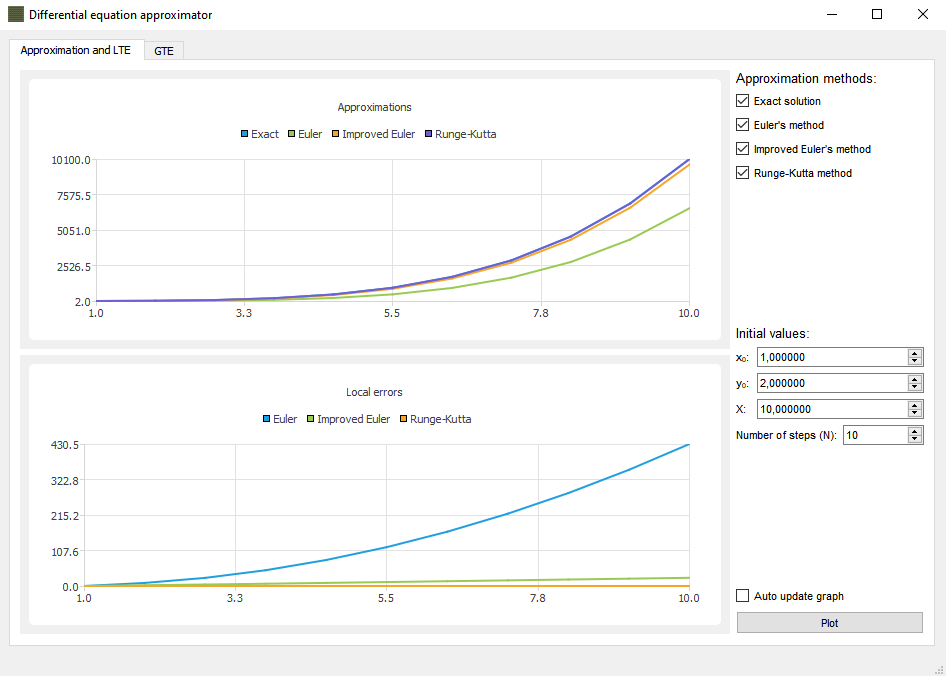
\includegraphics[scale=0.5]{DiffEqMethodsAndLte.png}

\subsection{UML Diagram}
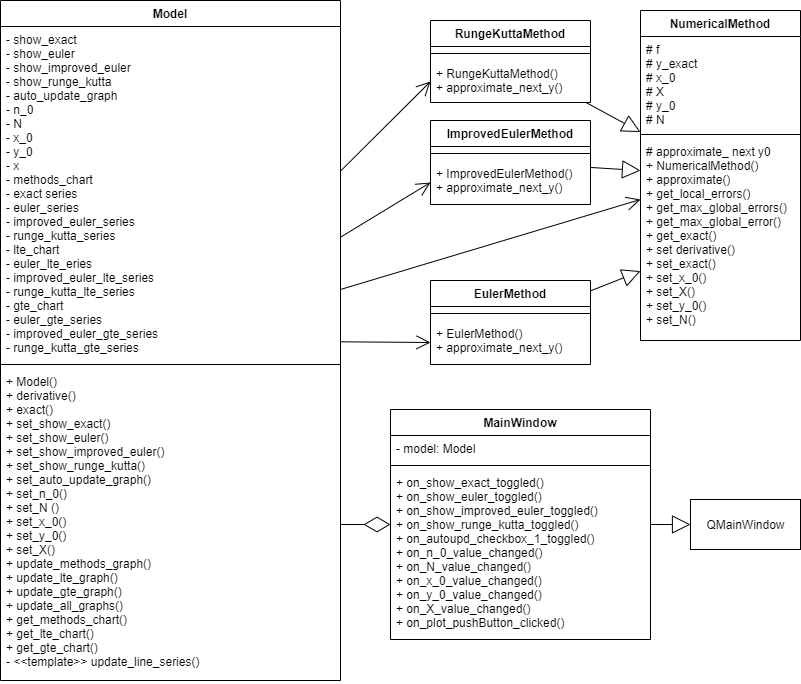
\includegraphics[scale=0.5]{DiffEqDiagram.png}

\subsection{The most interesting parts of source code}
These are the main methods for calculating approximations
\begin{minted}{c++}
QVector<QPointF> NumericalMethod::approximate() const{
    QVector<QPointF> result(N+1);
    result[0].rx() = x_0;
    result[0].ry() = y_0;
    double step = (X - x_0)/N;
    for (unsigned int i = 1; i < N+1; i++) {
        double x_prev = result[i-1].rx();
        double y_prev = result[i-1].ry();
        double x = x_0 + step*i;
        double y = approximate_next_y(x_prev, y_prev, step, f);
        result[i].rx() = x;
        result[i].ry() = y;
    }
    return result;
}

QVector<QPointF> NumericalMethod::get_local_errors() const {
    QVector<QPointF> result(N+1);
    result[0].rx() = x_0;
    result[0].ry() = 0;
    double step = (X - x_0)/N;
    for (unsigned int i = 1; i < N+1; i++) {
        double x_prev = result[i-1].rx();
        double x = x_0 + step*i;
        double error = fabs(y_exact(x, x_0, y_0) - approximate_next_y(x_prev, y_exact(x_prev, x_0, y_0), step, f));
        result[i].rx() = x;
        result[i].ry() = error;
    }
    return result;
}

QVector<QPointF> NumericalMethod::get_max_global_errors(unsigned int n_0)
{
    // use N_orig as N will change within the method
    // keep original value of N to restore it later
    unsigned int N_orig = N;

    QVector<QPointF> result(N_orig - n_0 + 1);
    for (unsigned int i = n_0; i <= N_orig; i++) {
        N = i;
        result[i-n_0].rx() = i;
        result[i-n_0].ry() = get_max_global_error();
    }

    N = N_orig;
    return result;
}

double NumericalMethod::get_max_global_error() const {
    auto approximation = approximate();

    double max_error = 0;
    double step = (X - x_0)/N;
    for (unsigned int i = 1; i < N+1; i++) {
        double x = x_0 + step*i;
        double error = fabs(y_exact(x, x_0, y_0) - approximation[i].ry());
        if (error > max_error) {
            max_error = error;
        }
    }
    return max_error;
}

QVector<QPointF> NumericalMethod::get_exact() const
{
    QVector<QPointF> result(N+1);
    result[0].rx() = x_0;
    result[0].ry() = y_0;
    double step = (X - x_0)/N;
    for (unsigned int i = 1; i < N+1; i++) {
        double x = x_0 + step*i;
        double y = y_exact(x, x_0, y_0);
        result[i].rx() = x;
        result[i].ry() = y;
    }
    return result;
}
\end{minted}
This is one of the overloadings of approximate\_next\_y (for Euler method)
\begin{minted}{c++}
double EulerMethod::approximate_next_y(double x_prev, double y_prev, double h, double (*f)(double, double)) const {
    return y_prev + h*f(x_prev, y_prev);
}
\end{minted}

\section{Part III}
\subsection{Plot created by the program (global errors)}
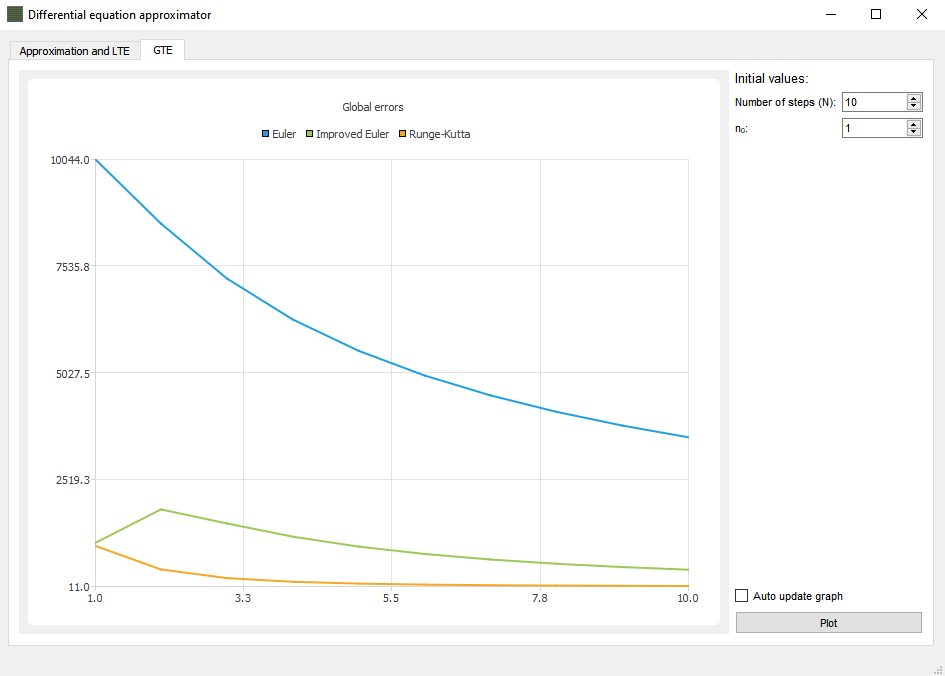
\includegraphics[scale=0.5]{DiffEqGte.png}

\end{document}
